\section{\method{}}
\label{sec:method}

\begin{figure*}[t]
\centering
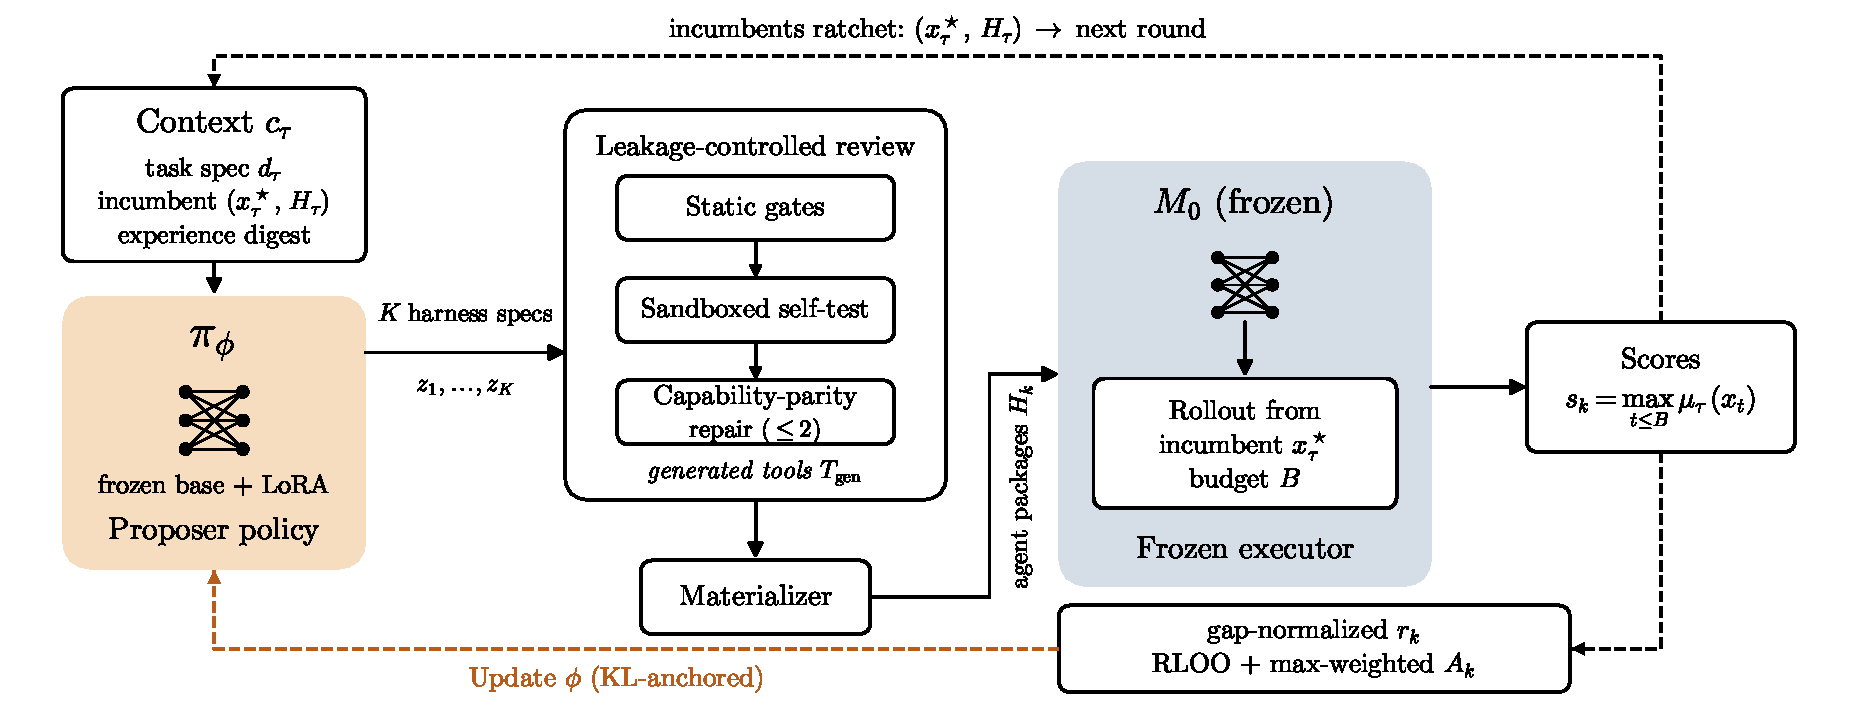
\includegraphics[width=\textwidth]{figures/overview_1.pdf}
\caption{\textbf{Overview of \method{}.}  \emph{Outer loop:} a proposer
$\pi_\phi$---the executor's own frozen base plus a LoRA adapter, the only
trained component---reads a task context $c_\tau$ (task spec, incumbent program
and harness, and a digest of what every previous candidate did, scored, and died
of) and emits $K$ harness specs.  Generated tool code passes a leakage-controlled
review chain (fail-closed static gates, sandboxed self-test, and repair held to
capability parity with the executor) before a deterministic materializer compiles
each spec into a runnable agent package $H_k$.  \emph{Inner loop:} the
permanently frozen executor $M_0$ rolls out each package from the incumbent
program under a hard evaluator budget $B$.  Two feedback paths close the loop:
the group's scores become gap-normalized rewards and RLOO advantages that update
\emph{only} $\phi$, and the round's best program and harness ratchet forward into
the next round's context.  Nothing in this loop updates $M_0$.}
\label{fig:overview}
\end{figure*}

\subsection{Setup and objective}
\label{sec:method-setup}

An agent is a pair $\Phi = (M, H)$ of a language model $M$ and a harness $H$.
We treat the harness as a concrete, typed object
$H = (P,\, S,\, D,\, \theta,\, T)$: a system prompt $P$; a skill package $S$
loaded into context; descriptions $D$ of the agent's tools (the behavioral
interface through which $M$ understands its own machinery); control parameters
$\theta$ (sampling temperature, iteration caps, middleware thresholds); and a
tool set $T = T_{\mathrm{fixed}} \cup T_{\mathrm{gen}}$, where
$T_{\mathrm{gen}}$ are \emph{generated} tools shipped as Python source and
compiled into the agent.  Prior scaffold optimization searches subsets of this
object---prompts~\citep{opro,gepa}, workflow graphs~\citep{aflow,agentsquare},
or agent code~\citep{adas,dgm}; we treat the full tuple as the output of a
learned policy.

A task $\tau = (d_\tau, x_0, \mu_\tau, B)$ consists of a natural-language
description, a seed program with an editable region, a black-box evaluator
returning a scalar score, and a hard budget of $B$ evaluator calls.  Running
$(M_0, H)$ on $\tau$ produces an edit$\to$evaluate trajectory whose outcome is
the best score reached within budget,
$s(\tau, H) = \max_{t \le B}\, \mu_\tau(x_t)$, where $x_t$ is the program
after $t$ edits from the round's start program.  Rounds inherit the incumbent rather than the seed
(\S\ref{sec:method-search}), so a valid candidate's score is floored at the
incumbent's and the reward below is non-negative except for invalid candidates.  The executor $M_0$ is frozen:
its weights never change, whether by fine-tuning or by test-time
training~\citep{ttt,ttrl}.  Improvement is delegated to a proposer
$\pi_\phi(z \mid c_\tau)$ that emits a harness spec $z$---compiled to $H_z$ by a
deterministic materializer---conditioned on a context $c_\tau$ holding
$d_\tau$, the incumbent best program and harness, and digested telemetry from
earlier rounds.  The learning problem is
\begin{equation}
\max_\phi \;\; \mathbb{E}_{\tau \sim \mathcal{T}} \;
\mathbb{E}_{z \sim \pi_\phi(\cdot \mid c_\tau)}
\big[\, s(\tau, H_z) \,\big],
\label{eq:objective}
\end{equation}
optimized with group-relative RL over $K$ proposer episodes per task per round.
What separates this formulation from per-task scaffold
search~\citep{adas,gepa,aflow,dgm} is the trained object: the \emph{proposer}
itself, so design knowledge amortizes across tasks and rounds instead of being
re-derived per task.  Like ADAS and the Darwin G\"odel Machine, and unlike
prompt- or graph-level search~\citep{gepa,aflow}, our search space carries
executable code, so the reachable harness family is not enumerable in advance.
Two more separate it from executor RL~\citep{grpo,agenticrl}: no gradient
touches $M_0$, and the reward is an \emph{outer} quantity---the best score of an
entire inner trajectory, not a per-token signal.

\emph{The core difficulty is credit assignment through two nested loops: a
scalar summarizing an entire frozen-executor rollout must teach the proposer
which of its design decisions---a prompt clause, a control parameter, a
generated tool---mattered, under evaluator noise and a rollout budget too small
to average it away.}  The rest of this section follows one round through the
system (Algorithm~\ref{alg:outer}): a typed spec space that makes decisions
legible (\S\ref{sec:method-genome}), a review chain that keeps generated code
from corrupting the measurement (\S\ref{sec:method-safety}), and a group
objective shaped for best-of-$K$ discovery (\S\ref{sec:method-rl}).

\subsection{The harness genome}
\label{sec:method-genome}
Candidates are expressed in a typed, fail-closed spec language rather than
free-form code: every submission either validates---and compiles into a
runnable package---or is rejected with a machine-readable error that flows
back into the proposer's next context.  \emph{Declarative} fields
reconfigure fixed machinery: the executor's system prompt, the skill
playbook, the descriptions of the fixed tools, sampling parameters, the
iteration cap, and middleware thresholds (budget reminders, stall-triggered
restarts, output truncation).  \emph{Generative} fields extend the machinery
itself: up to three \texttt{new\_tools}---each a name, description, JSON
input schema, and Python implementation---plus up to two new skills, up to two
\texttt{new\_middlewares} (a hook and a Python implementation each), and the
removal of designated optional tools.  Unlike tool-\emph{use}
pipelines~\citep{toolformer,toolllm} and library-induction methods that
abstract tools from solution traces~\citep{latm,creator,craft,trove,
voyager}, tools here are authored by the \emph{proposer} policy as part of a
harness, before the executor ever runs, and become first-class members of
the compiled agent.  A deterministic materializer turns a validated spec
into a complete package---prompt, skill files, tool schemas,
\texttt{custom\_tools/*.py} bound to a runtime dispatcher---so identical
specs yield byte-identical agents (modulo provenance metadata) and a spec hash de-duplicates candidates
within a group.

\paragraph{An experience-conditioned proposer.}
The proposer is itself a small agent: $\pi_\phi$ (frozen base plus LoRA)
runs inside a fixed two-tool harness (\texttt{validate\_spec},
\texttt{submit\_spec}) for one episode per candidate.  Its context $c_\tau$
carries the task description, an excerpt of the incumbent best program, the
incumbent spec and score, and an \emph{experience digest}: for every
candidate of the previous visit, its score, evaluator calls, stop reason,
changed fields, validation errors, and per-tool review outcomes, plus an
optional curated analyst note about the scoring rule
(\S\ref{sec:method-search}).  The $K$ episodes for a task share $c_\tau$ and
differ only in sampling seed, forming a single group for the group-relative update.  Feeding outcomes back
as language---rather than only as scalars---echoes reflective
optimization~\citep{reflexion,gepa,trace}; the difference is that here the
reflection loop trains a persistent policy, so design knowledge accumulates
in weights rather than in a per-task search state.

\subsection{Leakage-controlled tool generation}
\label{sec:method-safety}

Letting the proposer write code that runs inside the evaluation loop
invites the classic failure modes of specification
gaming~\citep{skalse2022,specgaming}: a tool that reads the evaluator or
answer files hacks the reward outright~\citep{denison2024,baker2025,
impossiblebench}, and a repair pathway routed through a strong model can
\emph{leak} solution knowledge into the executor's context, corrupting the
claim that the frozen executor did the discovering.  \method{} closes both
channels by construction, in four layers.
\textbf{(1) Capability surface:} a generated tool implements a single
\texttt{run(ctx, args)} entry point and touches the world only through
\texttt{ctx}---staged edits, cheap subsampled probes, budgeted evaluation,
task-input samples, scratch space.  The evaluator's implementation, the ground
truth, and the network are unreachable through this surface, and the static gates
below enforce the same boundary independently (the full capability surface is
listed in Appendix~\ref{app:sdk}).
\textbf{(2) Static gates:} a fail-closed AST pass enforces an import
whitelist, forbids \texttt{os}/\texttt{subprocess}/\texttt{open}/%
\texttt{exec}/dunder access, and requires the exact entry signature;
survivors execute against a mock context in an rlimit-sandboxed subprocess.
\textbf{(3) Capability-parity repair:} tools that fail enter a bounded
repair loop ($\le 2$ rounds) whose repairer is \emph{the same frozen served
model} as the executor---never a stronger external model---so the reviewer
cannot inject knowledge the executor lacks.  The repair prompt carries only
the code and the error (a scrubber rejects prompts containing evaluator or
target-score content), and a \emph{localization guard} rejects repairs whose
similarity to the original falls below $0.55$: a rewrite is treated as
attempted knowledge injection, not a fix.
\textbf{(4) Fail-closed accounting:} repaired code is re-gated and
re-tested; tools that never pass are dropped, and a candidate left without
any effective mutation is invalidated.  The review outcome of every tool is
reported back to the proposer in the next experience digest.

\subsection{A group objective for discovery}
\label{sec:method-rl}

Group-relative policy optimization was built for preference and
reasoning tuning, where rewards share a scale and the mean group outcome is
the target~\citep{grpo,rloo}.  Discovery violates both premises: scores live
on task-specific scales with a meaningful notion of \emph{remaining
headroom}, and the outer loop banks only the group's best rollout.  Per task
group of $K$ scores $\{s_k\}$, \method{} uses three modifications, each
motivated by an observed failure of the standard recipe
(\S\ref{sec:exp-results}, Obs.~4).
\textbf{Gap-normalized reward:} $g_k = (s_k - b_\tau)/(u_\tau - b_\tau)$,
the fraction of the remaining gap closed, where $b_\tau$ is the incumbent
best and $u_\tau$ a task ceiling.  We set $u_\tau$ to the published target score
for the task, which normalizes credit across heterogeneous scales; it enters the
\emph{reward} only, never the executor's context or the harness, and when no
target is available the reward falls back to relative gain over $b_\tau$.
Positive rewards are soft-capped as
$r_k = 3\tanh(g_k/3)$, which preserves the ranking among large gains where a
symmetric clip erases it.  Invalid candidates receive a fixed negative
reward.
\textbf{Leave-one-out baseline, no variance scaling:}
$A^{\mathrm{LOO}}_k = r_k - \frac{1}{K-1}\sum_{j\ne k} r_j$; dividing by the
group standard deviation---as in standard GRPO---amplifies $10^{-4}$-scale
evaluator noise into full-scale advantages in near-saturated groups.  (The
same term is independently implicated as a bias source by
\citet{drgrpo}; discovery's heterogeneous scales make the failure acute.)
\textbf{Max-weighted sharpening:} because deployment harvests
best-of-$K$~\citep{bond,infalign}, we interpolate toward the group-max
objective,
\begin{equation}
A_k \;=\; \alpha\Big(\sftm(r/T)_k - \tfrac{1}{K}\Big)
        \;+\; (1-\alpha)\, A^{\mathrm{LOO}}_k,
\label{eq:advantage}
\end{equation}
with $\alpha = 0.3$ and temperature $T$ set adaptively from the group's
reward range; the softmax term is a Monte-Carlo surrogate for the gradient
of the expected group maximum, while the RLOO term retains dense signal.
Degenerate groups are excluded outright: all-tied groups (which would teach
``any valid spec suffices''), sub-noise score differences (collapsed to
ties)---a guard family in the spirit of DAPO's dynamic filtering of uninformative
groups~\citep{dapo}.  Training is anchored by a KL penalty to the frozen
base policy, and every step's checkpoint is retained, so a validity collapse is
reverted by resuming from the previous step rather than trained through.

\subsection{Coupling RL to search}
\label{sec:method-search}

The RL loop optimizes the proposer; three mechanisms make the surrounding
campaign an effective search.  \textbf{Program inheritance:} rollouts start
from the incumbent best program rather than the seed, so rounds compound and
a candidate harness is credited only for \emph{surpassing} the incumbent;
displaced champions are archived as parents and shown to the executor as
alternative approaches from other basins.  \textbf{Cascade screening:} wide
rounds sample $K{=}16$ candidates under a cheap 5-call screen and promote
the top four to full budget---successive halving in the spirit of
bandit-based configuration search, and empirically our primary engine of new
program-family discovery.  \textbf{Telemetry and analyst notes:} the
experience digest upgrades the proposer from blind mutation to debugging.
Automated analyst briefs pass the same fail-closed leak guard as the repair
chain (claim-neutralizing and marker-dropping text transforms); a
\emph{curated} note may additionally expose structural facts about the
scoring rule, but it is a human channel the guard does not cover---a
protocol we audit rather than a mechanism we enforce.  The one violation we
found is disclosed and its result excluded (\S\ref{sec:exp-results},
Obs.~1).  Freezing the executor makes this ecosystem
analyzable: since $M_0$ never changes, every improvement decomposes into
what the proposer learned (\S\ref{sec:exp-results}, Obs.~2) and what the
search found (Obs.~3).

\begin{algorithm}[t]
\caption{One outer round of \method{}}
\label{alg:outer}
\begin{algorithmic}[1]
\Require frozen executor $M_0$; proposer $\pi_\phi$; tasks $\mathcal{T}$;
         incumbents $(H_\tau, x^\star_\tau)$; group size $K$
\For{each task $\tau \in \mathcal{T}$}
  \State build context $c_\tau$: task spec, $x^\star_\tau$ excerpt, incumbent
         spec/score, experience digest
  \State sample $K$ specs $z_k \sim \pi_\phi(\cdot \mid c_\tau)$
         \COMMENT{one proposer episode each}
  \For{each generated tool in each $z_k$}
    \State static gates $\to$ sandboxed self-test $\to$ ($\le 2$)
           capability-parity repairs; drop on failure
           \COMMENT{\S\ref{sec:method-safety}}
  \EndFor
  \State materialize valid specs into packages $H_k$; de-duplicate by spec hash
  \State roll out $(M_0, H_k)$ from $x^\star_\tau$; obtain scores $s_k$
         \COMMENT{cascade: screen, then promote}
  \State compute advantages by Eq.~\eqref{eq:advantage} against the pre-round
         incumbent; skip degenerate groups
  \State update $(H_\tau, x^\star_\tau)$ on strict improvement; archive parent
\EndFor
\State update $\phi$ with the advantages of Eq.~\eqref{eq:advantage} under a KL anchor; revert on validity collapse
\end{algorithmic}
\end{algorithm}
